% Appendix A
\chapter{Manifold learning algorithms for artificial data} % Main appendix title
\label{AppendixA} % For referencing this appendix elsewhere, use \ref{AppendixA}

\lhead{Appendix. \emph{Manifold learning algorithms for artificial data}} % This is for the header on each page - perhaps a shortened title

\begin{figure}[ht]
\begin{center}
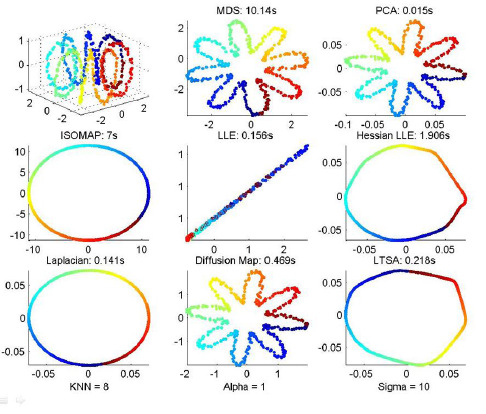
\includegraphics[width=\textwidth]{./Figures/App1.png}
\caption{ Manifold learning algorithms comparison using Swiss Roll. MDS and PCA fails to unroll Swiss Roll; LLE and Laplacian fails to perform too; Diffusion maps couldn't unroll Swiss Roll. }
%\label{pca}
\end{center}
\end{figure}


\begin{figure}[ht]
\begin{center}
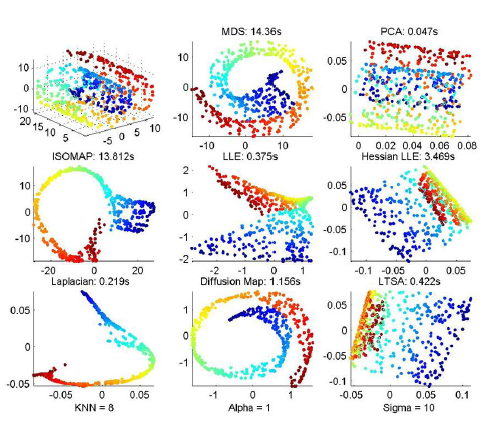
\includegraphics[width=\textwidth]{./Figures/App2.png}
\caption{ Manifold learning algorithms comparison using Toroidal Helix. ISOMAP, LLE, Laplacian, and Diffusion Map unraveled Toroidal Helix into a
circle, which is correct. PCA and MDS fails to perform. }
%\label{pca}
\end{center}
\end{figure}